\usepackage{wasysym}\usepackage{graphicx}\documentclass{article}
\usepackage[utf8]{inputenc}
\usepackage{float}
\usepackage[margin=1in]{geometry}
\usepackage{minted}
\usepackage{setspace}
\usepackage[parfill]{parskip}
\usepackage{graphicx}
\usepackage{minted}
\usepackage{pdflscape}

\usepackage{hyperref}
\hypersetup{
    colorlinks=true,
    linkcolor=black,
    filecolor=magenta,
    urlcolor=blue,
    pdfpagemode=FullScreen,
}

\renewcommand*\contentsname{Indholdsfortegnelse}
\renewcommand{\figurename}{Figur}
\renewcommand{\tablename}{Tabel}

\usepackage{subcaption}
\usepackage{icomma}

% TODO package:
\usepackage{lipsum}                     % Dummytext
\usepackage{xargs}                      % Use more than one optional parameter in a new commands
% \usepackage[pdftex,dvipsnames]{xcolor}
% 
\usepackage[colorinlistoftodos,prependcaption,textsize=tiny]{todonotes}
\newcommandx{\unsure}[2][1=]{\todo[linecolor=red,backgroundcolor=red!25,bordercolor=red,#1]{#2}}
\newcommandx{\change}[2][1=]{\todo[linecolor=blue,backgroundcolor=blue!25,bordercolor=blue,#1]{#2}}
\newcommandx{\info}[2][1=]{\todo[linecolor=OliveGreen,backgroundcolor=OliveGreen!25,bordercolor=OliveGreen,#1]{#2}}
\newcommandx{\improvement}[2][1=]{\todo[linecolor=Plum,backgroundcolor=Plum!25,bordercolor=Plum,#1]{#2}}
\newcommandx{\thiswillnotshow}[2][1=]{\todo[disable,#1]{#2}}
%

\definecolor{light-gray}{gray}{0.95}
\newcommand{\code}[1]{\colorbox{light-gray}{\texttt{#1}}}

\renewcommand{\baselinestretch}{1.25}

\graphicspath{ {./images/} }

\title{DAB 2 - Model 2}
\author{
    Magnus Mølgaard Christensen - 201807361
    \\Lasse Hyldahl Jensen - 201911335
    \\Jacob Røjgaard - 201710343
    \\DAB E21 gruppe 15
    \\Aarhus Universitet}

\date{16. November 2021}

\begin{document}
    \maketitle
    \newpage
    \begin{figure}[H]
        \centering
        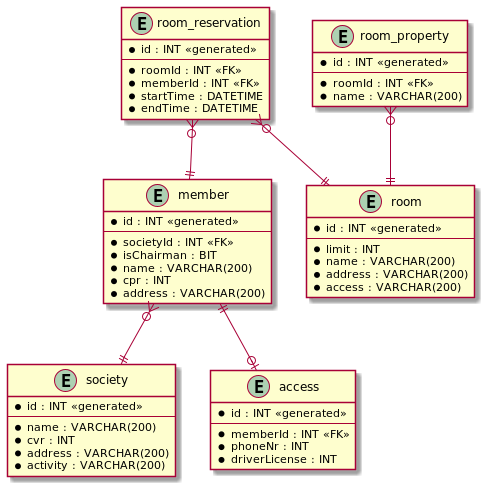
\includegraphics[height=10cm]{./er-diagram.png}
        \caption{E/R Diagram over den samlede implementering}
    \end{figure}
    
    \begin{figure}[H]
        \centering
        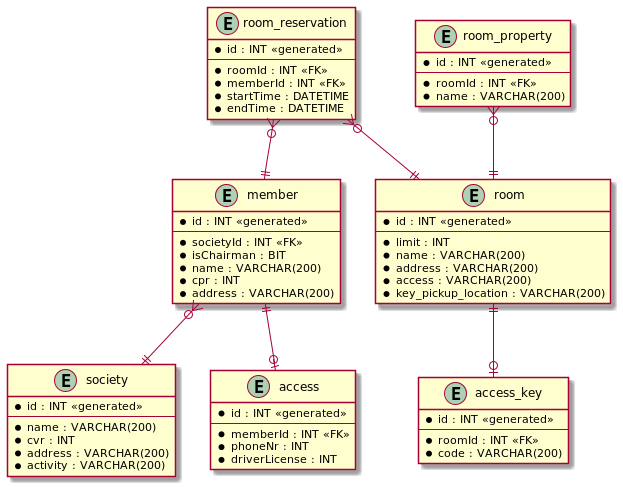
\includegraphics[height=10cm]{./er-diagram-with-migrations.png}
        \caption{E/R Diagram med nye krav}
    \end{figure}
    
\end{document}